\documentclass[aps,prb,reprint,superscriptaddress,twocolumn,floatfix]{revtex4-2}
\usepackage[utf8]{inputenc}
\usepackage{graphicx}
\usepackage{amsmath,amssymb}
\usepackage{bm}
\usepackage[colorlinks=true,linkcolor=blue,citecolor=blue,urlcolor=blue]{hyperref}
\graphicspath{{figures/}}
\newcommand{\Tc}{$T_c$}
\newcommand{\muS}{$\mu^{*}$}
\newcommand{\SI}[1]{Supplemental Material, Sec.~#1}

\begin{document}

\title{Compositional complexity does not raise $T_c$: an active-learning KKR-CPA search for bcc refractory high-entropy superconductors}

\author{Author}
\affiliation{Affiliation 1}
\author{Author 2}
\affiliation{Affiliation 2}

\date{\today}

\begin{abstract}
To be completed.
\end{abstract}

\maketitle

\section{Introduction}

High-entropy alloys (HEAs), solid solutions of five or more elements in near-equimolar
proportions~\cite{Yeh2004,Cantor2004}, were found to superconduct in 2014, when
Ko\v{z}elj \emph{et al.} reported $T_c = 7.3$~K in the bcc alloy
Ta$_{34}$Nb$_{33}$Hf$_8$Zr$_{14}$Ti$_{11}$~\cite{Kozelj2014}. Since then several dozen
bcc superconducting HEAs built from the group 4--7 transition metals have been
synthesised~\cite{SunCava2019,Kitagawa2020}. Their critical temperatures lie between 3 and
9~K. As a function of the valence electron count (VEC) they show a broad maximum near 4.7
electrons per atom, reminiscent of the Matthias rule of the crystalline transition-metal
alloys~\cite{Matthias1955,Hulm1961,lit_vonRohr_15926113}. The electron count alone, however,
does not determine \Tc: three bcc Nb--Ti--Zr--Hf alloys with the same VEC of 4.375 have
critical temperatures between 7.1 and 8.2~K, so that the elemental composition, and not
only the VEC, has to be regarded as the relevant variable~\cite{lit_Idczak_fnz7bzmw}. This
raises an obvious question: is there, somewhere in the vast composition space of these elements, a
multicomponent bcc alloy whose \Tc\ exceeds that of the best binary alloys, Nb--Zr
(11~K), Nb--Ti and Nb--Hf (about 10~K)~\cite{Hulm1961,Kushwaha2025}? Or does the
``high-entropy'' route only add disorder, which smears the Fermi-surface features that
favour superconductivity?

Answering this question by experiment is slow, and answering it by fully \emph{ab initio}
theory is very expensive. The quantitative theory of conventional superconductors requires the
Eliashberg function $\alpha^2F(\omega)$, i.e.\ the phonon spectrum and the electron--phonon
matrix elements of the alloy~\cite{Giustino2017,Baroni2001}. For a chemically disordered
solid solution this means large supercells, many phonon calculations and a statistical
average over configurations, so that a single composition costs days of computer time; a
systematic search over a ten-component simplex is out of reach. We therefore take a different
route. The KKR Green's-function method in the coherent-potential approximation
(KKR-CPA)~\cite{Korringa1947,KohnRostoker1954,Soven1967,Akai1989} treats substitutional
disorder in a single bcc unit cell. From its self-consistent potentials the McMillan--Hopfield
parameters $\eta_i$ of the components follow from the Gaspari--Gyorffy
formula~\cite{GaspariGyorffy1972,Papaconstantopoulos1977}, the electron--phonon coupling
$\lambda$ from $\eta$ and an estimate of the phonon frequencies~\cite{Hopfield1969}, and
\Tc\ from the McMillan equation~\cite{McMillan1968,AllenDynes1975}. This ``rigid-muffin-tin''
route was established for the elemental transition
metals~\cite{Papaconstantopoulos1977,Butler1977} and, combined with the CPA, has been used
for superconducting HEAs~\cite{Jaskiewicz2016,Jaskiewicz2019}; KKR-CPA electronic structure
has also served to interpret the measured superconducting parameters of bcc
HEAs~\cite{lit_Sobota_06184512,lit_Idczak_16175814,lit_Idczak_fnz7bzmw}. It reduces the
cost of one composition to about ten CPU-hours, which makes thousands of compositions
affordable.

Even then, the composition space is too large to be enumerated. A ten-element simplex sampled
with a 5\% step contains $\binom{29}{9} \approx 10^7$ compositions, far beyond a brute-force
scan. We therefore use active learning: a machine-learning surrogate trained on the calculated
alloys proposes the next compositions to calculate, balancing exploitation of the
best-known region against exploration of regions where the surrogate is
uncertain~\cite{Srinivas2010,Lakshminarayanan2017}. Machine learning has so far
entered the theory of superconductors mostly as a regression tool, e.g.\ to predict \Tc\ from
the chemical formula on the basis of experimental databases~\cite{Stanev2018} or to improve
the analytic \Tc\ formulas with the help of Eliashberg solutions~\cite{Xie2022}. Its role here
is different: the surrogate only guides the search, and every \Tc\ that we report is
calculated by the KKR-CPA pipeline.

We apply this scheme to two sets of ten elements, with and without the 3$d$ metals V and
Sc, and determine the highest calculated \Tc\ as a function of the minimum number of
constituents imposed on the alloy. All compositions are assumed to form a random bcc solid
solution. This is an assumption of the study and not a result of it; its consistency is
examined a posteriori by comparing the total energies of the bcc, fcc and hcp phases of the
optimal compositions. The estimator is validated beforehand against the published critical
temperatures of bcc alloys of the same elements.

\section{Element sets and known superconductors}
\label{sec:sets}

We consider two sets of ten elements. Set~A, \{Ti, Nb, Zr, Hf, Ta, Mo, W, Y, Re, Ru\},
contains the 4$d$ and 5$d$ refractory metals of groups 4--8 together with Ti and Y.
Set~B, \{Ti, Nb, Zr, Hf, Ta, Mo, W, Y, V, Sc\}, replaces the two heaviest elements by
the 3$d$ metals V and Sc; V-containing bcc HEAs are common in the
literature~\cite{lit_Ishizu_19102275,lit_Sharma_s9064801}, and Sc-containing ones have
been reported recently~\cite{lit_Sobota_06184512,lit_Sobota_50351820}. Eight elements are
shared, so the two sets test whether a 3$d$ admixture changes the picture.

Table~S1 of the Supplemental Material lists the 121 published \Tc\ values of bcc
alloys whose constituents belong to set A, to set B or to both (100 distinct
compositions from 42 papers in set B, 65 compositions from 33 papers in set A; 65 entries
belong to both sets). Within this compilation, which is extensive but may not
be complete, the highest \Tc\ in set~A is 9.4~K for
Nb$_{67}$Hf$_{11}$Zr$_{11}$Ti$_{11}$~\cite{lit_vonRohr_15926113}, followed by Nb-rich
(TiHfTa)$_{1-x}$Nb$_x$ alloys with 8.8--9.1~K~\cite{lit_Li_ad9fa8}. Among the alloys with V
or Sc the highest values are 8.4~K for Sc--Nb--Ti--Zr, reported for a multiphase
sample~\cite{lit_Krnel_15031122}, and 7.2~K for the V-containing
(NbV)$_{0.67}$(HfZrTi)$_{0.33}$~\cite{lit_vonRohr_15926113}. All of them lie below the binary maxima of the same elements: 11.1~K
for Nb$_{0.85}$Zr$_{0.15}$, 9.7~K for Nb$_{0.85}$Ti$_{0.15}$ and 9.8~K for
Nb$_{0.85}$Hf$_{0.15}$ in as-cast samples~\cite{Kushwaha2025}, consistent with the
classic survey of Hulm and Blaugher~\cite{Hulm1961}.

\section{Method}
\label{sec:method}

\subsection{KKR-CPA estimate of $T_c$}

Every composition is treated as a random bcc solid solution with the KKR-CPA code
AkaiKKR (\textsc{Machikaneyama})~\cite{Akai1989}, in the scalar-relativistic approximation,
with the PBE exchange--correlation functional~\cite{PerdewBurkeErnzerhof1996}, $s$, $p$,
$d$ and $f$ scattering channels, a $0.6$~Ry energy window and a muffin-tin potential. The
estimate of \Tc\ rests on the rigid-muffin-tin
approximation~\cite{GaspariGyorffy1972,Papaconstantopoulos1977,Butler1977}, used before for a
superconducting HEA in Refs.~\cite{Jaskiewicz2016,Jaskiewicz2019}. Here it is implemented as
a fully automated procedure with no composition-dependent input, which consists of three
stages.
(i)~The equilibrium lattice constant $a_0$ and bulk modulus follow from a Birch--Murnaghan
fit to total energies on a scan of lattice constants within $\pm 5\%$ of the
concentration-averaged elemental value, with 256 $k$-points in the irreducible wedge of
the Brillouin zone. (ii)~A final self-consistent calculation at $a_0$ with 1661 $k$-points
in the irreducible wedge gives the partial densities of states and the radial wave
functions at the Fermi energy, from which the McMillan--Hopfield parameter of each
component is evaluated with the Gaspari--Gyorffy formula~\cite{GaspariGyorffy1972},
\begin{equation}
  \eta_i = \frac{E_F}{\pi^2 N(E_F)} \sum_l 2(l+1)\,
  \sin^2(\delta_{l+1}^{i} - \delta_{l}^{i})\,
  \frac{n_l^{i}\, n_{l+1}^{i}}{n_l^{(1)}\, n_{l+1}^{(1)}},
  \label{eq:gg}
\end{equation}
with the scattering phase shifts $\delta_l^i$, the partial densities of states $n_l^i$ of
component $i$, the free-scatterer densities $n_l^{(1)}$ and the total density of states
$N(E_F)$ per spin obtained from the Lloyd formula~\cite{Lloyd1967}. A comparison with published
McMillan--Hopfield parameters is given in \SI{S2}. The alloy parameter is the concentration average,
$\eta = \sum_i x_i \eta_i$~\cite{Jaskiewicz2016}. (iii)~The coupling constant is
\begin{equation}
  \lambda = \frac{\eta}{M\langle\omega^2\rangle},\qquad
  \langle\omega^2\rangle = \tfrac{3}{5}\,(k_B\theta_D/\hbar)^2 ,
  \label{eq:lambda}
\end{equation}
with the average atomic mass $M = \sum_i x_i M_i$ and the Debye temperature of the
alloy. KKR-CPA total energies of strained cells give the shear constants $C'$ and
$C_{44}$ and hence a Debye temperature, but for the Zr-, Hf- and Ti-rich alloys this
$\theta_D^{\rm KKR}$ is spuriously low because the static bcc lattice is close to
mechanical instability (\SI{S3}). We therefore use the concentration average of the
elemental Debye temperatures, $\theta_D^{\rm mix} = \sum_i x_i \theta_{D,i}$, in
Eq.~(\ref{eq:lambda}), and the McMillan equation~\cite{McMillan1968}
\begin{equation}
  T_c = \frac{\theta_D^{\rm mix}}{1.45}
  \exp\!\left[-\frac{1.04(1+\lambda)}{\lambda - \mu^*(1+0.62\lambda)}\right]
  \label{eq:mcmillan}
\end{equation}
with a single Coulomb pseudopotential $\mu^* = 0.1$ for all alloys. This value is at the
lower end of those used in the literature, which range from 0.1 to above 0.2 for
transition-metal alloys (\SI{S9}). It is not derived but calibrated: it is the value for
which the median ratio of calculated to measured \Tc\ over the literature set is close to
one (1.05 for set~A) and the mean absolute error is smallest. The choice of $\mu^*$ sets the
absolute scale of \Tc\ but has almost no effect on the ordering of the alloys (\SI{S9}) and
does not change the trends reported below (\SI{S10}). One composition costs about ten CPU-hours on a 28-core node.

\subsection{Correction for V and Sc (set B)}
\label{sec:corr}

With the parameters above, the alloys containing V or Sc are described much worse than the
rest: for the 47 literature entries with V or Sc the rank correlation between calculated
and measured \Tc\ drops to $\tau = 0.16$, against $0.66$ for the alloys without these elements.
Two physical effects, both specific to the 3$d$ metals, are missing from the rigid-muffin-tin
picture. First, V and Ti--V alloys are close to a ferromagnetic instability and their
\Tc\ is suppressed by spin fluctuations~\cite{Berk1966,RietschelWinter1979,Matin2014}:
McMillan-type estimates without paramagnons give about 20~K for Ti--V alloys, several times
the measured value~\cite{Matin2014}, and our uncorrected pipeline reproduces this
overestimate (17--21~K along the Ti--V line, \SI{S6}; 20.1~K for the V$_{68}$Ti$_{32}$
alloy that the uncorrected set-B optimisation selects as its best binary). The
spin-fluctuation mass enhancement of V and Nb is of the order of
0.2~\cite{RietschelWinter1979}. Second, Sc is an hcp metal whose tabulated Debye temperature (355~K) refers
to the hcp phase; the bcc phase relevant for the solid solution is much softer, and our own
KKR-CPA elastic constants give $\theta_D \approx 190$--220~K for bcc Sc (193~K at the
$k$-mesh of the pipeline). We therefore use for set~B
the corrected estimator $T_c^{\rm corr}$ in which (i) $\theta_{D,{\rm Sc}} = 215$~K enters
$\theta_D^{\rm mix}$, with $\lambda$ rescaled accordingly by
Eq.~(\ref{eq:lambda}), and (ii) an electron--paramagnon coupling
$\lambda_{\rm sf} = x_{\rm V}\,\alpha_{\rm V}\, s\ln[1/(1-s)]$, with the Stoner factor
$s = I_{\rm V} N_{\rm V}(E_F)$ of the V site and $\alpha_{\rm V} = 0.4$, is inserted into
the McMillan equation in the form proposed by Bose~\cite{Bose2009},
$1+\lambda \to 1+\lambda+\lambda_{\rm sf}$ and
$\lambda-\mu^* \to \lambda-\lambda_{\rm sf}-\mu^*$. The two parameters (215~K, 0.4) were
fitted to the V- and Sc-containing literature alloys; for compositions without V and Sc,
$T_c^{\rm corr}$ is identical to Eq.~(\ref{eq:mcmillan}). The correction is admittedly
empirical, and we show the set-B results both with and without it. Since set~A contains
neither V nor Sc, the correction does not affect any of the set-A results.

\subsection{Validation against experiment}
\label{sec:validation}

\begin{figure*}
  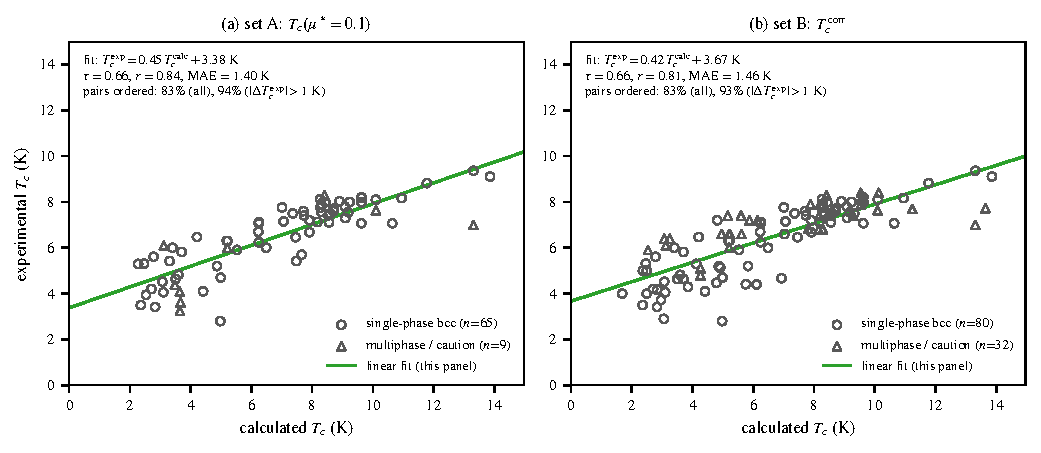
\includegraphics[width=\textwidth]{fig_validation}
  \caption{Measured versus calculated \Tc\ for the literature bcc alloys of (a) set~A and (b)
  set~B (corrected estimator of Sec.~\ref{sec:corr}). Every point is a separate published
  measurement, recomputed from scratch with the pipeline of Sec.~\ref{sec:method} (the same
  code and parameters as in the optimisation). Circles: single-phase bcc samples; triangles:
  samples reported as multiphase or otherwise flagged in the source. The line in each panel
  is a linear fit to all points of that panel. $\tau$ is Kendall's rank correlation, $r$
  Pearson's correlation, and ``pairs ordered'' the fraction of alloy pairs whose experimental
  order is reproduced.}
  \label{fig:validation}
\end{figure*}

Figure~\ref{fig:validation} compares the pipeline with the 121 literature values of
Table~S1; every alloy was calculated from scratch with exactly the code and parameters
used later in the optimisation. For set~A (74 entries) the mean absolute error is
1.40~K, the bias $+0.33$~K and Pearson's $r = 0.84$. A linear fit of the measured to
the calculated values, made separately for each set, has a slope of 0.45 (0.42 for set~B),
i.e.\ the calculation spreads the alloys over a wider \Tc\ range than experiment. We have no
quantitative explanation of this slope. Calculated coupling constants that exceed the
experimental ones have been reported for individual
HEAs~\cite{Jaskiewicz2016,lit_Sobota_06184512,lit_Idczak_fnz7bzmw}, and the approximations
made here, i.e.\ the neglect of local lattice distortions, the composition-independent
$\mu^*$ and the mixture rule for the phonon energy scale, may all contribute.

The optimisation described in Sec.~\ref{sec:optimiser} only has to decide which of two
compositions has the higher \Tc, so for our purpose the ordering of the alloys matters more
than the absolute error. Taking two alloys
of the literature set at random, the pipeline predicts which of them has the higher \Tc\
correctly in 83\% of the pairs (set~A, Kendall's $\tau = 0.66$). Many of the wrongly
ordered pairs differ by a few tenths of a kelvin, which is within the scatter of the
measurements themselves; restricting the comparison to pairs whose measured \Tc\ differ by more
than 1~K, the ordering is reproduced in 94\% of the cases. For the single-phase bcc entries
alone the numbers are 85\% and 95\%. For set~B with the corrected estimator the
corresponding values are 83\% and 93\% (112 entries, MAE 1.46~K, $r = 0.81$); without
the correction they fall to 73\% and 80\% ($\tau = 0.46$, Fig.~S1).

As a second test, which is closer to the question we ask, we calculated the binary lines
Nb--Zr, Nb--Ti and Nb--Hf (Fig.~S2). Experimentally, Nb--Zr is the
binary with the highest \Tc\ of all transition-metal solid solutions~\cite{Hulm1961};
recent as-cast Nb$_{0.85}X_{0.15}$ samples give 11.1~K for $X$ = Zr against 9.7~K (Ti) and
9.8~K (Hf)~\cite{Kushwaha2025}. The calculation reproduces this ordering: the Nb--Zr line
has a broad maximum of 19.0~K at Nb$_{60}$Zr$_{40}$, while Nb--Ti and Nb--Hf decrease
monotonically from the Nb-rich end, where they coincide within 0.1~K (13.9~K at $x = 0.1$).
Rescaled with the linear fit of Fig.~\ref{fig:validation}(a), which was obtained without
any binary alloy, the calculated values become 10.9--11.6~K for Nb--Zr and 9.4--9.7~K
(Ti) and 9.2--9.7~K (Hf) at $x = 0.1$--0.2, within 0.4~K of the measurements at $x = 0.15$.

The present estimate of \Tc\ has a limitation that restricts the scope of the search. The
\Tc\ of the transition-metal alloys has a second maximum at a valence electron count of about
6.4 per atom (Mo--Re)~\cite{Hulm1961}, and this maximum is not reproduced: the thirteen
literature alloys with at least 20\% of Mo, W and Re together are underestimated by a
median factor of 0.76 (1.04 for the remaining alloys), and the Re-containing ones by
factors of 0.4--0.6 (Table~S1). The search reported below is therefore a search around the
first maximum, at a valence electron count of about 4.7.

\subsection{Initial dataset}
\label{sec:init}

The optimiser starts from a random dataset computed with the same pipeline:
about 1800 compositions for each set. About 1000 of them are drawn
uniformly from the interior of the ten-dimensional simplex (a flat Dirichlet distribution).
Such points contain all ten elements, most of them in small amounts; a uniform sample of
the simplex practically never produces a binary or a ternary alloy. Since the alloys with
few components are exactly the ones we want to compare with, the dataset is complemented
with about 100 points on each $k$-dimensional face of the simplex, $k = 2, \dots, 9$:
for each point a random subset of $k$ elements is chosen (all 45 binary subsets are visited
at least once), the fractions of these elements are drawn from a flat Dirichlet distribution
truncated to $x_i \geq 0.05$, and the remaining elements are set to zero. In total the initial
sets contain 100 binaries, 100 ternaries, and so on. The best initial points are the
binaries Nb$_{\sim 60}$Zr$_{\sim 40}$ with 18.8 and 18.7~K in sets A and B
(\SI{S5}).

\subsection{Active-learning optimiser}
\label{sec:optimiser}

The compositions of the initial dataset are the starting point of an optimisation whose
aim is to find the compositions with the highest calculated \Tc. The objective is the \Tc\ of
Eq.~(\ref{eq:mcmillan}) (for set~B with the correction of Sec.~\ref{sec:corr}; the
optimisation without the correction is discussed in \SI{S6}). Each optimisation run is a loop
in which (i) a surrogate model is trained on all compositions calculated so far, (ii) the
surrogate scores a large pool of candidate compositions, and (iii) ten new compositions,
selected as described below, are calculated with the KKR-CPA pipeline and added to the data.

The surrogate is an ensemble of ten gradient-boosted regression-tree models
(CatBoost~\cite{Prokhorenkova2018}; depth 6, learning rate 0.03, early stopping on a 20\%
validation split), each trained on a different random 50\% subsample of the known data. For
a candidate composition the ten models give ten predictions of \Tc; we denote their mean by
$\mu$ and their standard deviation by $\sigma$, and use $\sigma$ as a measure of the
uncertainty of the prediction~\cite{Lakshminarayanan2017}. Following the common practice of
describing a material by statistics of the properties of its
constituents~\cite{Ward2016,Stanev2018}, the input of the models consists of the ten
concentrations and about forty descriptors derived from them: the concentration-weighted
means, variances and mean pairwise differences of the valence electron count, the number of
$d$ electrons, the atomic radius and the electronegativity of the constituents, the
atomic size mismatch, and the configurational entropy
$-\sum_i x_i \ln x_i$~\cite{Zhang2008}.

In every iteration $10^5$ candidate compositions are generated from three sources: 70\%
uniformly over the simplex (Sobol sequence), 10\% on random faces of the simplex, and 20\% in
the neighbourhood of the twenty best known compositions (each concentration of such a
composition is shifted by a Gaussian random number of standard deviation 0.03, and the
result is renormalised). The candidates are ranked by the score
$a = \mu + \beta\sigma$ with $\beta = 2$~\cite{Srinivas2010}. The first term favours the
region that the surrogate currently predicts to be the best. The second term favours
compositions for which the ten models disagree, which happens where the calculated data
are sparse or where \Tc\ varies rapidly with composition, i.e.\ exactly where a new
calculation is most informative; $\beta$ sets the balance between the two.
Candidates closer than 0.02 (Euclidean distance in composition space) to an already
calculated composition are discarded, and the ten compositions to be calculated are chosen
one after another, the score of each next one being increased in proportion to its distance
from the compositions already chosen or calculated. Both measures prevent the ten new
calculations of an iteration from being spent on nearly identical compositions.

Two constraints define the search space: no element may exceed 70\%, and the alloy must
contain at least $k$ elements with fractions above 5\%. The second constraint is the handle
by which we control the compositional complexity: a run with $k = 2$ may end in a binary, a
run with $k = 7$ must find the best alloy with at least seven substantial constituents. Each
$k$ is a completely independent run starting from the same initial dataset; the run with
$k = 5$ does not know the result of $k = 4$. A run stops when fifteen consecutive iterations
bring no improvement of the best valid composition; the runs reported below took 16--48
iterations, i.e.\ 160--480 KKR-CPA calculations each. Test runs with other values of $\beta$
(between 0 and 10) and with an initial set containing no face points end at the same
compositions, with \Tc\ within 0.2~K, and runs with $\mu^* = 0.2$ lead to compositions of the
same family (\SI{S6}), so the result does not depend on these settings of the
optimisation.

\section{Results}
\label{sec:results}

\begin{figure*}
  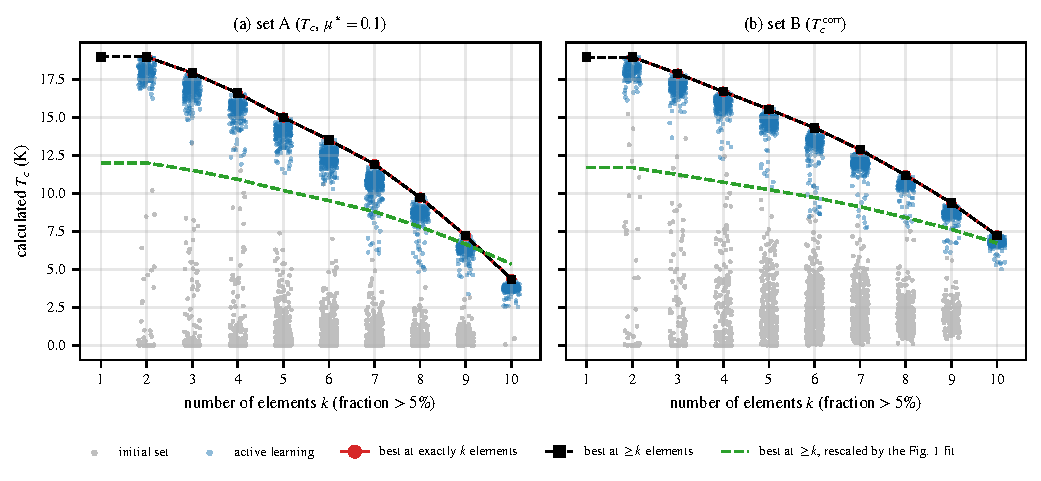
\includegraphics[width=\textwidth]{fig_pareto}
  \caption{Best \Tc\ calculated with KKR-CPA as a function of the number of constituent elements (fraction
  above 5\%) for (a) set~A and (b) set~B, pooled over all compositions evaluated in the nine
  runs with $k = 2, \dots, 10$ (grey: initial dataset, blue: compositions proposed by
  the optimiser). Circles: best composition with exactly $k$ elements; squares: best with at
  least $k$ elements. Green dashed line: the best \Tc\ at $\geq k$ elements rescaled with the
  linear fit of the corresponding panel of Fig.~\ref{fig:validation}, a rough estimate of the
  \Tc\ to be expected in experiment.}
  \label{fig:pareto}
\end{figure*}

\begin{figure*}
  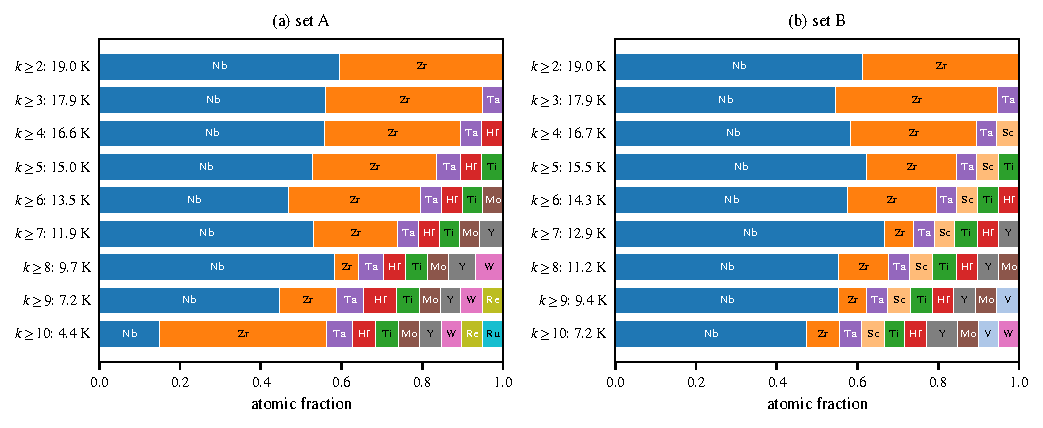
\includegraphics[width=\textwidth]{fig_champions}
  \caption{Composition of the best alloy found in each run, for (a) set~A and (b) set~B
  (with $T_c^{\rm corr}$). The label gives the imposed minimum number of elements $k$ and
  the \Tc\ of the champion calculated with KKR-CPA (not rescaled to experiment). Each element
  has the same colour in both panels. In no run does the champion contain more elements above
  5\% than required, although the constraint allows it.}
  \label{fig:champions}
\end{figure*}

Figure~\ref{fig:pareto} shows every composition evaluated in the nine independent runs per
element set against its number of constituents, and the resulting Pareto front of \Tc\
versus complexity. Figure~\ref{fig:champions} shows the champion of each run. Three
observations summarise the outcome.

\emph{The best alloy is the binary Nb--Zr, and every forced element costs \Tc.}
All \Tc\ values in this section are the values calculated with KKR-CPA from
Eq.~(\ref{eq:mcmillan}); as shown in Sec.~\ref{sec:validation}, they reproduce the
ordering of the measured alloys but not their absolute \Tc\ (the slope of the linear fit is
about 0.45 instead of 1).
The best \Tc\ with at least $k$ elements is 19.0, 17.9, 16.6, 15.0, 13.5, 11.9, 9.7, 7.2 and
4.4~K for $k = 2, \dots, 10$ in set~A, and 19.0, 17.9, 16.7, 15.5, 14.3, 12.9, 11.2, 9.4 and
7.2~K in set~B. The decrease is monotonic and nearly linear, 1.8~K per element in set~A and
1.5~K in set~B. Rescaled with the linear fits of Fig.~\ref{fig:validation}, the front
becomes 12.0~K at $k = 2$ and 5.4~K at $k = 10$ in set~A (11.7 and 6.7~K in set~B; green line
in Fig.~\ref{fig:pareto}). This rescaling is a crude simplification, a fit to alloys with
measured \Tc\ below 10~K applied to the whole front, and the numbers should be read only as an
estimate of what experiment can be expected to give, not as predictions. The best binaries, Nb$_{59}$Zr$_{41}$ (set A) and Nb$_{61}$Zr$_{39}$ (set B),
are the calculated optimum of the Nb--Zr line (Fig.~S2), and the best
ternaries, Nb$_{56}$Zr$_{39}$Ta$_5$ and Nb$_{54}$Zr$_{40}$Ta$_5$, are the same binary with the
smallest admissible admixture of Ta. No point in Fig.~\ref{fig:pareto}, from either the
random initial set or the active-learning proposals, lies above the binary optimum.

\emph{The forced elements enter at the 5\% floor, in a reproducible order.} In all champions
with $k \geq 3$ the majority elements are Nb (45--67\%) and Zr, and the remaining
constituents sit at 5--8\%, i.e.\ at the smallest fraction that satisfies the constraint
(Fig.~\ref{fig:champions}); the only exception is the ten-component champion of set~A,
in which Zr (41\%) rather than Nb is the majority element. The optimiser thus keeps every
additional element at the lowest fraction allowed: the elements beyond Nb and Zr are
present because the constraint requires them, not because they raise \Tc. The order in which they
are admitted is nearly the same in both sets and in the runs with $\mu^* = 0.2$ of \SI{S6}: Ta
first, then Hf and Ti, then Mo and Y, then W, and only when unavoidable Re and Ru (set~A)
or V (set~B). Since each run is independent, this order is a
property of the KKR-CPA \Tc\ landscape, a ranking of the elements by how little they reduce
the Nb--Zr coupling. In set~B the correction of Sec.~\ref{sec:corr} makes Sc the first element
admitted after Ta: with $\theta_{D,{\rm Sc}} = 215$~K, 5--6\% of Sc lowers
$\theta_D^{\rm mix}$ and raises $\lambda$ enough to add about 0.9~K relative to the same
alloy with Hf or Ti instead, which is why the set-B front lies 0.1--2.9~K above the set-A
front for $k \geq 4$. Without the correction the set-B champions for $k = 4$--7 contain V
at the floor instead of Sc, and the front is within 0.6~K of set~A up to $k = 7$
(Fig.~S3); for $k \geq 8$ set~B stays 1--3~K above set~A with or without the correction,
simply because set~A must then admit Re and Ru, which lower \Tc\ the most, whereas
set~B admits V and Sc. The part of the difference that rests on the empirical Sc correction,
which the six single-phase Sc alloys of the literature set do not support unambiguously,
should not be over-interpreted. The decrease of the front with $k$ does not depend on the
correction: without it the best \Tc\ at $\geq k$ elements in set~B is 20.1, 17.9, 16.7,
15.4, 14.1, 12.5, 11.0, 9.4 and 7.3~K for $k = 2, \dots, 10$. The only qualitative change is
at $k = 2$, where the uncorrected calculation prefers V$_{68}$Ti$_{32}$, an alloy of the
Ti--V line whose \Tc\ it overestimates (Sec.~\ref{sec:corr}); with the correction the best
binary is Nb--Zr, as in set~A.

\emph{\Tc\ is governed by $\lambda$ alone.} Over the optimised compositions the correlation
between $\lambda$ and \Tc\ is 0.998 (set~A) and 0.98 (set~B). The champions' $\lambda$ decreases
from 1.14 ($k = 2$) to 0.54 ($k = 10$) in set~A while $\theta_D^{\rm mix}$ rises only from
273 to 317~K (Fig.~S5). Each element added to Nb--Zr dilutes the Nb--Zr $d$-band
contribution to $\eta$, and the stiffer elements (Mo, W, Re, Ru) raise
$\langle\omega^2\rangle$ in the denominator of Eq.~(\ref{eq:lambda}); both lower $\lambda$.
The optimiser is also strikingly local: 91--100\% of the compositions it proposes come from
the neighbourhood of the current best alloys, and the gain over the best valid point of the
initial set grows from 0.2~K at $k = 2$ (the binary optimum is already in the initial set)
to 3--6~K at $k = 6$--8 and to 3.9~K at $k = 10$ in set~A; in set~B the initial set
contained no valid ten-component point at all.

\section{Thermodynamic stability}
\label{sec:td}

\begin{table*}
\caption{Structural and thermodynamic stability of the champions of Fig.~\ref{fig:champions},
from KKR-CPA total energies with the same settings as the lattice optimisation. $\Delta E_{\rm
fcc}$ and $\Delta E_{\rm hcp}$ are the energies of the fcc and hcp solid solutions above the bcc
one; $\Delta H_{\rm bcc}$ is the mixing enthalpy of the bcc alloy with respect to the bcc
elements, $\Delta H_{\rm gs}$ with respect to the elements in their KKR ground-state
structure; $S_{\rm conf} = -\sum_i x_i \ln x_i$; $\Delta G = \Delta H_{\rm bcc} - T k_B S_{\rm
conf}$ at $T = 1500$~K, the order of the freezing temperature of the as-cast samples. $T_c$ is the value calculated with KKR-CPA, $T_c^{\rm resc}$ the same value rescaled with the linear fit of
the corresponding panel of Fig.~\ref{fig:validation} (a rough estimate of the experimental \Tc). All
energies in meV/atom. The reference energies of W and Re, whose valence band is not fully
enclosed by the 0.6~Ry energy window, were computed with a 1.0~Ry window (\SI{S8}).}
\label{tab:td}
\begin{ruledtabular}
\begin{tabular}{clcrrrrrrrr}
set & $k$ & composition & $T_c$ (K) & $T_c^{\rm resc}$ (K) & $\Delta E_{\rm fcc}$ & $\Delta E_{\rm hcp}$ &
$\Delta H_{\rm bcc}$ & $\Delta H_{\rm gs}$ & $S_{\rm conf}/k_B$ & $\Delta G_{1500}$ \\
\hline
A & 2 & Nb$_{59}$Zr$_{41}$ & 19.0 & 12.0 & 220 & 247 & +73 & +75 & 0.68 & -14 \\
A & 3 & Nb$_{56}$Zr$_{39}$Ta$_{5}$ & 17.9 & 11.5 & 225 & 253 & +76 & +78 & 0.84 & -33 \\
A & 4 & Nb$_{56}$Zr$_{34}$Hf$_{5}$Ta$_{5}$ & 16.6 & 10.9 & 220 & 249 & +79 & +88 & 1.00 & -50 \\
A & 5 & Nb$_{53}$Zr$_{31}$Ta$_{6}$Ti$_{5}$Hf$_{5}$ & 15.0 & 10.2 & 206 & 236 & +103 & +113 & 1.18 & -49 \\
A & 6 & Nb$_{47}$Zr$_{33}$Ta$_{5}$Hf$_{5}$Mo$_{5}$Ti$_{5}$ & 13.5 & 9.5 & 220 & 248 & +105 & +115 & 1.33 & -67 \\
A & 7 & Nb$_{53}$Zr$_{21}$Y$_{6}$Ta$_{5}$Hf$_{5}$Ti$_{5}$Mo$_{5}$ & 11.9 & 8.8 & 227 & 254 & +152 & +165 & 1.43 & -33 \\
A & 8 & Nb$_{58}$Y$_{7}$W$_{7}$Ta$_{6}$Zr$_{6}$Hf$_{6}$Ti$_{5}$Mo$_{5}$ & 9.7 & 7.8 & 300 & 329 & +160 & +174 & 1.49 & -32 \\
A & 9 & Nb$_{45}$Zr$_{14}$Hf$_{8}$Ta$_{7}$Ti$_{6}$W$_{5}$Re$_{5}$Y$_{5}$Mo$_{5}$ & 7.2 & 6.7 & 296 & 323 & +126 & +152 & 1.80 & -106 \\
A & 10 & Zr$_{41}$Nb$_{15}$Ta$_{6}$Ti$_{6}$Hf$_{6}$Y$_{5}$Re$_{5}$Ru$_{5}$W$_{5}$Mo$_{5}$ & 4.4 & 5.4 & 228 & 245 & +124 & +174 & 1.92 & -124 \\
B & 2 & Nb$_{61}$Zr$_{39}$ & 19.0 & 11.7 & 228 & 254 & +72 & +74 & 0.67 & -15 \\
B & 3 & Nb$_{54}$Zr$_{40}$Ta$_{5}$ & 17.9 & 11.2 & 219 & 247 & +78 & +80 & 0.85 & -33 \\
B & 4 & Nb$_{58}$Zr$_{31}$Sc$_{6}$Ta$_{5}$ & 16.7 & 10.7 & 209 & 237 & +103 & +108 & 0.99 & -25 \\
B & 5 & Nb$_{62}$Zr$_{22}$Sc$_{5}$Ti$_{5}$Ta$_{5}$ & 15.5 & 10.2 & 221 & 250 & +114 & +120 & 1.09 & -27 \\
B & 6 & Nb$_{58}$Zr$_{22}$Ti$_{5}$Sc$_{5}$Ta$_{5}$Hf$_{5}$ & 14.3 & 9.7 & 200 & 229 & +123 & +135 & 1.26 & -40 \\
B & 7 & Nb$_{67}$Zr$_{7}$Ti$_{6}$Ta$_{5}$Y$_{5}$Hf$_{5}$Sc$_{5}$ & 12.9 & 9.1 & 222 & 251 & +161 & +176 & 1.23 & +2 \\
B & 8 & Nb$_{55}$Zr$_{12}$Ti$_{6}$Sc$_{6}$Ta$_{5}$Y$_{5}$Hf$_{5}$Mo$_{5}$ & 11.2 & 8.4 & 214 & 241 & +173 & +188 & 1.53 & -25 \\
B & 9 & Nb$_{55}$Zr$_{7}$Sc$_{6}$V$_{6}$Ti$_{6}$Mo$_{5}$Y$_{5}$Hf$_{5}$Ta$_{5}$ & 9.4 & 7.6 & 225 & 253 & +229 & +245 & 1.62 & +20 \\
B & 10 & Nb$_{47}$Zr$_{8}$Y$_{8}$Sc$_{6}$Ta$_{6}$Hf$_{5}$Mo$_{5}$W$_{5}$Ti$_{5}$V$_{5}$ & 7.2 & 6.7 & 227 & 255 & +261 & +278 & 1.84 & +24 \\

\end{tabular}
\end{ruledtabular}
\end{table*}

The search was restricted to the bcc lattice. For the 18 champions of
Fig.~\ref{fig:champions} we checked a posteriori that this restriction is consistent, by
computing with the same KKR-CPA settings the total energy of the fcc solid solution, optimised
over the lattice constant, and of the hcp solid solution, optimised over the lattice constant
and $c/a$ (Table~\ref{tab:td}). In every case bcc is the lowest structure, by 200--300~meV/atom with
respect to fcc and by 230--330~meV/atom with respect to hcp. For comparison, the same
calculation gives $+393$ and $+417$~meV/atom for pure Nb, and correctly finds hcp as the
ground state of Ti, Zr, Hf, Y, Sc and Ru. For the compositions found by the optimiser
the assumption of a bcc lattice made during the search is therefore self-consistent: neither
the fcc nor the hcp solid solution has a lower energy. In this respect the champions behave
like the measured HEAs of Table~S1, which crystallise in the bcc structure.

The mixing enthalpies $\Delta H_{\rm bcc}$ are positive for all champions: $+73$~meV/atom for
Nb$_{59}$Zr$_{41}$ and between $+76$ and $+261$~meV/atom for the other champions.
Referring the elements to their ground-state structures instead of bcc changes these
numbers by 2--25~meV/atom, and by 50~meV/atom for the ten-component champion of set~A, which
contains Ru and Re, whose hcp ground state lies far below bcc. The bcc solid solutions are thus not ground states but
high-temperature phases stabilised by the configurational entropy: at 1500~K, $T k_B S_{\rm
conf}$ (90--250~meV/atom) outweighs $\Delta H_{\rm bcc}$ for all set-A champions and for six
of the nine set-B champions; of the other three, the seven-component one is within
3~meV/atom of zero and the nine- and ten-component ones lie at $+20$ and $+24$~meV/atom. This is
the usual situation of the refractory HEA superconductors, which are arc-melted and quenched
and retain the bcc solid solution metastably; the positive $\Delta H$ of Nb--Zr is
consistent with its well-known bcc miscibility gap. Our calculation does not address
the decomposition into several bcc phases or the formation of intermetallics, and the
$\Delta G$ values should be read only as a statement that the single-phase bcc solution
is accessible at the synthesis temperature, not as a prediction of its low-temperature
stability.

\section{Conclusions}
\label{sec:conclusions}

To be completed.

\begin{acknowledgments}
To be completed.
\end{acknowledgments}

\bibliography{refs}

\end{document}
